% !TEX encoding = UTF-8 Unicode
\chapter{Login}

\section{目的}
练习cookie和session的使用,加深对它们的理解。
\section{目标}
使用cookie和session为项目增加登陆功能。
\section{过程}
\subsection{使用Session实现登陆}
\begin{enumerate}
\item
前台界面

如Figure \ref{login1}所示,此前台界面位于content\_left.jsp这个div内。
\begin{figure}
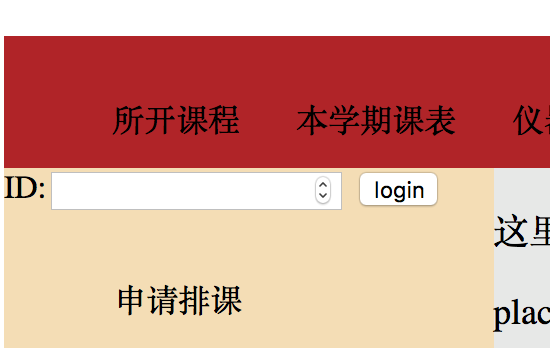
\includegraphics{Login1}
\caption{Login界面}
\label{login1}
\end{figure}
\item
前台代码

如Figure \ref{login2}所示。注意这里使用了\emph{EL和JSTL}表达式。

\begin{figure}
\begin{verbatim}
<!--content_left.jsp-->
<%@ taglib prefix="c" uri="http://java.sun.com/jsp/jstl/core" %>
<div class="content left">
<c:choose>
<c:when test="${not empty sessionScope.userName }">
你好,${sessionScope.userName }。
<form action="logout.jsp" method="post">
			<input type="submit" value="logout"></form>
</c:when>
<c:otherwise>
<form action="Login" method="post">
		ID:<input type="number" min=20060001 name="id">
		<input type="submit" value="login">
		</form>
</c:otherwise>
</c:choose>
\end{verbatim}
\caption{根据session信息决定如何显示登陆信息的代码}
\label{login2}
\end{figure}

\item
控制登陆的servlet

其代码如Figure \ref{login3}所示。
\begin{figure}
\begin{lstlisting}
//Login.java
protected void doPost(HttpServletRequest request, HttpServletResponse response) 
  throws ServletException, IOException {
	int id = Integer.parseInt(request.getParameter("id"));
	Db db = new Db();
	Connection conn = db.getConnection();
	String sql = "select name from teachers where id=?";
	try {
		PreparedStatement pst = conn.prepareStatement(sql);
		pst.setInt(1, id);
		ResultSet rs=pst.executeQuery();
		if(rs.next()) {
			String name = rs.getString(1);
			HttpSession s = request.getSession();
			s.setAttribute("id", id);
			s.setAttribute("userName", name);
			response.sendRedirect("index.jsp");
		}else {
			PrintWriter out = response.getWriter();
			out.print("Wrong ID!\nWill return to index.");
			response.setHeader("refresh","3;URL=index.jsp");
		}
		
	} catch (SQLException e) {
		e.printStackTrace();
	} finally {
		try {
			conn.close();
		} catch (SQLException e) {
			// TODO Auto-generated catch block
			e.printStackTrace();
		}
	}
}
\end{lstlisting}
\caption{负责处理登陆的servlet部分代码}
\label{login3}
\end{figure}
\item
注销

用户登陆之后要给其提供主动注销的功能,因为这里的登陆是通过session来实现的,所以要达到注销的目的,只需要使session无效即可。可以设置一个按钮,点下此按钮会提交一个post请求到logout.jsp页面,在logout.jsp页面中调用session.invalidate(),使session变得无效。
\end{enumerate}
\subsection{Cookie和Session配合实现登陆}
使用Session登陆后,其有效期范围为一次会话过程,如果关闭浏览器之后,Session就会消失了(只是服务器和客户端对应不起来了)。当客户端再打开网站时,服务器以为又是一个新的用户来访问了,就又开启一个Session,用户需要重新登陆。怎么让服务器能够知道是某个用户再次访问本网站而不是一个新用户来访问的呢?答案是可以结合Cookie技术来实现。

默认情况下,tomcat会将Session的生存周期设置为30分钟,如若想修改,请参照Figure \ref{login4}的代码。
\begin{figure}
\begin{verbatim}
$tomcat_home$/conf/web.xml
<!-- ==================== Default Session Configuration ================= -->
 602   <!-- You can set the default session timeout (in minutes) for all newly -->
 603   <!-- created sessions by modifying the value below.    -->
 604   <!-- default: 30-->
 605 
 606     <session-config>
 607         <session-timeout>30</session-timeout>
 608     </session-config>

\end{verbatim}
\caption{tomcat的Session默认生存周期}
\label{login4}
\end{figure}

在Figure \ref{login3}中,我们将登陆后的用户名保存在了Session里,为了确保这个用户在一定的时间范围内即使关闭浏览器再打开浏览器来访问本网站也不需要重新登陆,我们需要做的就是把这个Session id写到Cookie里面发送给客户端。客户端下次再访问本网站的时候,自动带上Cookie,tomcat服务器端会自动检查是否有一个叫JSESSIONID的Cookie,如果有,就和服务器上的JSESSIONID进行比较,如果查找到了匹配的,那服务器就知道是某个特定的用户再次来访问了,服务器就会自动的取出那个特定Session相关的数据。这里还需要把Cookie的生命周期设置一下,以免关闭浏览器后Cookie失效。具体代码如Figure \ref{login5}所示。
\begin{figure}
\begin{verbatim}
//Login.java
HttpSession s = request.getSession();
s.setAttribute("id", id);
s.setAttribute("userName", name);
Cookie ck = new Cookie("JSESSIONID",s.getId());
ck.setMaxAge(600);
response.addCookie(ck);
\end{verbatim}
\caption{tomcat的Session默认生存周期}
\label{login5}
\end{figure}
